\documentclass[11pt,oneside]{article}
\usepackage[T1]{fontenc}
\usepackage[utf8]{inputenc}
% \usepackage{lmodern}
%\usepackage[adobe-utopia,uppercase=upright,greeklowercase=upright]{mathdesign}
\usepackage[adobe-utopia]{mathdesign}
%\usepackage{minionpro}
% \usepackage{pifont}
% \usepackage{amssymb}
\usepackage{amsmath}
\usepackage[francais]{babel}
% \usepackage[francais]{varioref}
\usepackage[dvips]{graphicx}

\usepackage{framed}
\usepackage[normalem]{ulem}
\usepackage{fancyhdr}
\usepackage{titlesec}
\usepackage{vmargin}
\usepackage{longtable}

\usepackage{ifthen}


%\usepackage{epsfig}
\usepackage{subfig}

\usepackage{multirow}
\usepackage{multicol} % Portions de texte en colonnes
\usepackage{flafter}%floatants après la référence



\usepackage{color}
\usepackage{colortbl}


\definecolor{gris25}{gray}{0.75}
\definecolor{bleu}{RGB}{18,33,98}
\definecolor{bleuf}{RGB}{42,94,171}
\definecolor{bleuc}{RGB}{231,239,247}
\definecolor{rougef}{RGB}{185,18,27}
\definecolor{rougec}{RGB}{255,230,231}
\definecolor{vertf}{RGB}{103,126,82}
\definecolor{vertc}{RGB}{220,255,191}

\newenvironment{rem}[1][\hsize]%
{%
    \def\FrameCommand
    {%
\rotatebox{90}{\textit{\textsf{Remarque}}} 
        {\color{bleuf}\vrule width 3pt}%
        \hspace{0pt}%must no space.
        \fboxsep=\FrameSep\colorbox{bleuc}%
    }%
    \MakeFramed{\hsize#1\advance\hsize-\width\FrameRestore}%
}%
{\endMakeFramed}%


\newenvironment{savoir}[1][\hsize]%
{%
    \def\FrameCommand
    {%
\rotatebox{90}{\textit{\textsf{Savoir}}} 
        {\color{bleuf}\vrule width 3pt}%
        \hspace{0pt}%must no space.
        \fboxsep=\FrameSep\colorbox{bleuc}%
    }%
    \MakeFramed{\hsize#1\advance\hsize-\width\FrameRestore}%
}%
{\endMakeFramed}%

\newenvironment{prob}[1][\hsize]%
{%
    \def\FrameCommand%
    {%
\rotatebox{90}{\textit{\textsf{ Problématique}}} 
        {\color{rougef}\vrule width 3pt}%
        \hspace{0pt}%must no space.
        \fboxsep=\FrameSep\colorbox{rougec}%
    }%
    \MakeFramed{\hsize#1\advance\hsize-\width\FrameRestore}%
}%
{\endMakeFramed}%

\newenvironment{obj}[1][\hsize]%
{%
    \def\FrameCommand%
    {%
\rotatebox{90}{\textit{\textsf{ $\;$}}} 
        {\color{rougef}\vrule width 3pt}%
        \hspace{0pt}%must no space.
        \fboxsep=\FrameSep\colorbox{rougec}%
    }%
    \MakeFramed{\hsize#1\advance\hsize-\width\FrameRestore}%
}%
{\endMakeFramed}%

\newenvironment{defi}[1][\hsize]%
{%
    \def\FrameCommand%
    {%
\rotatebox{90}{\textit{\textsf{Définition\\}}} 
        {\color{bleuf}\vrule width 3pt}%
        \hspace{0pt}%must no space.
        \fboxsep=\FrameSep\colorbox{bleuc}%
    }%
    \MakeFramed{\hsize#1\advance\hsize-\width\FrameRestore}%
}%
{\endMakeFramed}%


\newenvironment{hypo}[1][\hsize]%
{%
    \def\FrameCommand%
    {%
\rotatebox{90}{\textit{\textsf{Hypothèse\\}}} 
        {\color{bleuf}\vrule width 3pt}%
        \hspace{0pt}%must no space.
        \fboxsep=\FrameSep\colorbox{bleuc}%
    }%
    \MakeFramed{\hsize#1\advance\hsize-\width\FrameRestore}%
}%
{\endMakeFramed}%


\newenvironment{prop}[1][\hsize]%
{%
    \def\FrameCommand%
    {%
\rotatebox{90}{\textit{\textsf{Propriété\\}}} 
        {\color{bleuf}\vrule width 3pt}%
        \hspace{0pt}%must no space.
        \fboxsep=\FrameSep\colorbox{bleuc}%
    }%
    \MakeFramed{\hsize#1\advance\hsize-\width\FrameRestore}%
}%
{\endMakeFramed}%

\newenvironment{props}[1][\hsize]%
{%
    \def\FrameCommand%
    {%
\rotatebox{90}{\textit{\textsf{Propriétés\\}}} 
        {\color{bleuf}\vrule width 3pt}%
        \hspace{0pt}%must no space.
        \fboxsep=\FrameSep\colorbox{bleuc}%
    }%
    \MakeFramed{\hsize#1\advance\hsize-\width\FrameRestore}%
}%
{\endMakeFramed}%

\newenvironment{exemple}[1][\hsize]%
{%
    \def\FrameCommand%
    {%
\rotatebox{90}{\textit{\textsf{Exemple\\}}} 
        {\color{vertf}\vrule width 3pt}%
        \hspace{0pt}%must no space.
        \fboxsep=\FrameSep\colorbox{vertc}%
    }%
    \MakeFramed{\hsize#1\advance\hsize-\width\FrameRestore}%
}%
{\endMakeFramed}%

\newenvironment{resultat}[1][\hsize]%
{%
    \def\FrameCommand%
    {%
\rotatebox{90}{\textit{\textsf{Résultat\\}}} 
        {\color{rougef}\vrule width 3pt}%
        \hspace{0pt}%must no space.
        \fboxsep=\FrameSep\colorbox{rougec}%
    }%
    \MakeFramed{\hsize#1\advance\hsize-\width\FrameRestore}%
}%
{\endMakeFramed}%

\newenvironment{methode}[1][\hsize]%
{%
    \def\FrameCommand%
    {%
\rotatebox{90}{\textit{\textsf{Méthode\\}}} 
        {\color{rougef}\vrule width 3pt}%
        \hspace{0pt}%must no space.
        \fboxsep=\FrameSep\colorbox{rougec}%
    }%
    \MakeFramed{\hsize#1\advance\hsize-\width\FrameRestore}%
}%
{\endMakeFramed}%

\newenvironment{theo}[1][\hsize]%
{%
    \def\FrameCommand%
    {%
\rotatebox{90}{\textit{\textsf{Théorème\\}}} 
        {\color{rougef}\vrule width 3pt}%
        \hspace{0pt}%must no space.
        \fboxsep=\FrameSep\colorbox{rougec}%
    }%
    \MakeFramed{\hsize#1\advance\hsize-\width\FrameRestore}%
}%
{\endMakeFramed}%

\newenvironment{warn}[1][\hsize]%
{%
    \def\FrameCommand%
    {%
\rotatebox{90}{\textit{\textsf{Attention\\}}} 
        {\color{rougef}\vrule width 3pt}%
        \hspace{0pt}%must no space.
        \fboxsep=\FrameSep\colorbox{rougec}%
    }%
    \MakeFramed{\hsize#1\advance\hsize-\width\FrameRestore}%
}%
{\endMakeFramed}%

% \usepackage{pstricks}
%\usepackage{minitoc}
% \setcounter{minitocdepth}{4}

\setcounter{tocdepth}{2}

% \mtcselectlanguage{french} 

%\usepackage{draftcopy}% "Brouillon"
% \usepackage{floatflt}
\usepackage{psfrag}
%\usepackage{listings} % Permet d'insérer du code de programmation
\renewcommand{\baselinestretch}{1.2}

% Changer la numérotation des figures :
% ------------------------------------
% \makeatletter
% \renewcommand{\thefigure}{\ifnum \c@section>\z@ \thesection.\fi
%  \@arabic\c@figure}
% \@addtoreset{figure}{section}
% \makeatother
 


%%%%%%%%%%%%
% Définition des vecteurs %
%%%%%%%%%%%%
 \newcommand{\vect}[1]{\overrightarrow{#1}}

%%%%%%%%%%%%
% Définition des torseusr %
%%%%%%%%%%%%

 \newcommand{\torseur}[1]{%
\left\{{#1}\right\}
}

\newcommand{\torseurcin}[3]{%
\left\{\mathcal{#1} \left(#2/#3 \right) \right\}
}

\newcommand{\torseurstat}[3]{%
\left\{\mathcal{#1} \left(#2\rightarrow #3 \right) \right\}
}

 \newcommand{\torseurc}[8]{%
%\left\{#1 \right\}=
\left\{
{#1}
\right\}
 = 
\left\{%
\begin{array}{cc}%
{#2} & {#5}\\%
{#3} & {#6}\\%
{#4} & {#7}\\%
\end{array}%
\right\}_{#8}%
}

 \newcommand{\torseurcol}[7]{
\left\{%
\begin{array}{cc}%
{#1} & {#4}\\%
{#2} & {#5}\\%
{#3} & {#6}\\%
\end{array}%
\right\}_{#7}%
}

 \newcommand{\torseurl}[3]{%
%\left\{\mathcal{#1}\right\}_{#2}=%
\left\{%
\begin{array}{l}%
{#1} \\%
{#2} %
\end{array}%
\right\}_{#3}%
}

 \newcommand{\vectv}[3]{%
\vect{V\left( {#1} \in {#2}/{#3}\right)}
}


\newcommand{\vectf}[2]{%
\vect{R\left( {#1} \rightarrow {#2}\right)}
}

\newcommand{\vectm}[3]{%
\vect{\mathcal{M}\left( {#1}, {#2} \rightarrow {#3}\right)}
}


 \newcommand{\vectg}[3]{%
\vect{\Gamma \left( {#1} \in {#2}/{#3}\right)}
}

 \newcommand{\vecto}[2]{%
\vect{\Omega\left( {#1}/{#2}\right)}
}
% }$$\left\{\mathcal{#1} \right\}_{#2} =%
% \left\{%
% \begin{array}{c}%
%  #3 \\%
%  #4 %
% \end{array}%
% \right\}_{#5}}

%  ------------------------------------------
% | Modification du formatage des sections : | 
%  ------------------------------------------

% Grands titres :
% ---------------

\newcommand{\titre}[1]{%
\begin{center}
      \bigskip
      \rule{\textwidth}{1pt}
      \par\vspace{0.1cm}
      
      \textbf{\large #1}
      \par\rule{\textwidth}{1pt}
    \end{center}
    \bigskip
  }

% Supprime le numéro du chapitre dans la numérotation des sections:
% -----------------------------------------------------------------
\makeatletter
\renewcommand{\thesection}{\@arabic\c@section}
\makeatother


% \titleformat{\chapter}[display]
% {\normalfont\Large\filcenter}
% {}
% {1pc}
% {\titlerule[1pt]
%   \vspace{1pc}%
%   \Huge}[\vspace{1ex}%
% \titlerule]


%%%% Chapitres Comme PY Pechard %%%%%%%%%
% numéro du chapitre
\DeclareFixedFont{\chapnumfont}{OT1}{phv}{b}{n}{80pt}
% pour le mot « Chapitre »
\DeclareFixedFont{\chapchapfont}{OT1}{phv}{m}{it}{40pt}
% pour le titre
\DeclareFixedFont{\chaptitfont}{T1}{phv}{b}{n}{25pt}

\definecolor{gris}{gray}{0.75}
\titleformat{\chapter}[display]%
	{\sffamily}%
	{\filleft\chapchapfont\color{gris}\chaptertitlename\
	\\
	\vspace{12pt}
	\chapnumfont\thechapter}%
	{16pt}%
	{\filleft\chaptitfont}%
	[\vspace{6pt}\titlerule\titlerule\titlerule]

%%%%  Fin Chapitres Comme PY Pechard %%%%%%%%%


% Section, subsection, subsubsection sans serifs :
% % ----------------------------------------------

% \makeatletter
% \renewcommand{\section}{\@startsection{section}{0}{0mm}%
% {\baselineskip}{.3\baselineskip}%
% {\normalfont\sffamily\Large\textbf}}%
% \makeatother

\makeatletter
\renewcommand{\@seccntformat}[1]{{\textcolor{bleu}{\csname
the#1\endcsname}\hspace{0.5em}}}
\makeatother

\makeatletter
\renewcommand{\section}{\@startsection{section}{1}{\z@}%
                       {-4ex \@plus -1ex \@minus -.4ex}%
                       {1ex \@plus.2ex }%
                       {\normalfont\Large\sffamily\bfseries}}%
\makeatother
 
\makeatletter
\renewcommand{\subsection}{\@startsection {subsection}{2}{\z@}
                          {-3ex \@plus -0.1ex \@minus -.4ex}%
                          {0.5ex \@plus.2ex }%
                          {\normalfont\large\sffamily\bfseries}}
\makeatother
 
\makeatletter
\renewcommand{\subsubsection}{\@startsection {subsubsection}{3}{\z@}
                          {-2ex \@plus -0.1ex \@minus -.2ex}%
                          {0.2ex \@plus.2ex }%
                          {\normalfont\large\sffamily\bfseries}}
\makeatother
 
\makeatletter             
\renewcommand{\paragraph}{\@startsection{paragraph}{4}{\z@}%
                                    {-2ex \@plus-.2ex \@minus .2ex}%
                                    {0.1ex}%               
{\normalfont\sffamily\bfseries}}
\makeatother
 
\makeatletter
\renewcommand{\subparagraph}{\@startsection{subparagraph}{5}{\z@}%
                                       {-2ex \@plus-.1ex \@minus .2ex}%
                                       {0.1ex}%
				    {\normalfont\normalsize\sffamily\bfseries}}
\makeatletter
% \makeatletter
% \renewcommand{\subsection}{\@startsection{subsection}{1}{2mm}%
% {\baselineskip}{.3\baselineskip}%
% {\normalfont\sffamily\large\textbf}}%
% \makeatother
% 
% \makeatletter
% \renewcommand{\subsubsection}{\@startsection{subsubsection}{2}{4mm}%
% {\baselineskip}{.15\baselineskip}%
% {\normalfont\sffamily\large\textbf}}%
% \makeatother
% 
% \makeatletter
% \renewcommand{\paragraph}{\@startsection{paragraph}{3}{6mm}%
% {\baselineskip}{.15\baselineskip}%
% {\normalfont\sffamily\large\textbf}}%
% \makeatother
 
\setcounter{secnumdepth}{4}


%  --------
% | Marges |
%  --------


% \setmarginsrb{2.5cm}{1.5cm}{2.5cm}{2cm}{1cm}{1cm}{1cm}{1cm}
\setmarginsrb{1.5cm}{1cm}{1cm}{1.5cm}{1cm}{1cm}{1cm}{1cm}

% Changer les marges localement :
% -----------------------------
\newenvironment{changemargin}[2]{\begin{list}{}{%
\setlength{\topsep}{0pt}%
\setlength{\leftmargin}{0pt}%
\setlength{\rightmargin}{0pt}%
\setlength{\listparindent}{\parindent}%
\setlength{\itemindent}{\parindent}%
\setlength{\parsep}{0pt plus 1pt}%
\addtolength{\leftmargin}{#1}%
\addtolength{\rightmargin}{#2}%
}\item }{\end{list}}



\usepackage{pst-solides3d}
\usepackage{titletoc}
\titlecontents{chapter}[+3pc]
  {\addvspace{10pt}\sffamily\bfseries}
{\contentslabel[{\pscirclebox[fillstyle=solid,fillcolor=gray!25,
linecolor=gray!25,framesep=4pt]{\textcolor{white}{\thecontentslabel}}}]{2.5pc}}
  {}
  {\dotfill \normalfont\thecontentspage\ }

\titlecontents{section}[3pc]
  {\addvspace{2pt}\sffamily}
  {\contentslabel[\thecontentslabel]{1.8pc}}
  {}
  {\dotfill \normalfont\thecontentspage\ }

\titlecontents{subsection}[5pc]
  {\addvspace{2pt}\sffamily}
  {\contentslabel[\thecontentslabel]{1.8pc}}
  {}
  {\dotfill \normalfont\thecontentspage\ }

\titlecontents{subsubsection}[8pc]
  {\addvspace{2pt}\sffamily}
  {\contentslabel[\thecontentslabel]{3pc}}
  {}
  {\dotfill \normalfont\thecontentspage\ }
%{\;\titlerule\;\normalfont\thecontentspage\ }

\titlecontents{paragraph}[9pc]
  {\addvspace{2pt}\sffamily}
  {\contentslabel[\thecontentslabel]{3.5pc}}
  {}
  {\dotfill \normalfont\thecontentspage\ }



\usepackage[raccourcis]{FAST}
\usepackage[%
    pdftitle={Produits Procédés Matériaux --  Mise en forme des matériaux},
    pdfauthor={Xavier Pessoles},
    colorlinks=true,
    linkcolor=blue,
    citecolor=magenta]{hyperref}
\usepackage{schemabloc}



% \makeatletter \let\ps@plain\ps@empty \makeatother
%% DEBUT DU DOCUMENT
%% =================
\sloppy
\hyphenpenalty 10000

\newcommand{\Pointilles}[1][3]{%
\multido{}{#1}{\makebox[\linewidth]{\dotfill}\\[\parskip]
}}


\colorlet{shadecolor}{orange!15}

\newtheorem{theorem}{Theorem}


\begin{document}


\newboolean{prof}
\setboolean{prof}{true}
%------------- En tetes et Pieds de Pages ------------
\pagestyle{fancy}
\renewcommand{\headrulewidth}{0pt}

\fancyhead{}
\fancyhead[L]{%
\noindent\noindent\begin{minipage}[c]{2.6cm}
%Lycée Rouvière PTSI

\includegraphics[width=2cm]{png/logo_ptsi.png}%
\end{minipage}
}

\fancyhead[C]{\rule{12cm}{.5pt}}

\fancyhead[R]{%
\noindent\begin{minipage}[c]{3cm}
\begin{flushright}
\footnotesize{\textit{\textsf{Sciences Industrielles\\ pour l'Ingénieur}}}%
\end{flushright}
\end{minipage}
}

\renewcommand{\footrulewidth}{0.2pt}

\fancyfoot[C]{\footnotesize{\bfseries \thepage}}
\fancyfoot[L]{\footnotesize{2012 -- 2013} \\ X. \textsc{Pessoles}}
\ifthenelse{\boolean{prof}}{%
\fancyfoot[R]{\footnotesize{Cours -- CI 6 : PPM -- P}}
}{%
\fancyfoot[R]{\footnotesize{Cours -- CI 6 : PPM}}
}



\begin{center}
 \huge\textsc{CI 6 -- PPM -- Produits Procédés Matériaux}

 \large\textsc{Élaboration des pièces mécaniques. Introduction de la chaîne numérique.}
\end{center}

\begin{center}
 \LARGE\textsc{Chapitre 3 -- Mise en forme des matériaux}
\end{center}

\begin{flushright}
\textit{D'après documents de Jean-Pierre Pupier}
\end{flushright}

\vspace{.5cm}



\begin{minipage}[c]{.2\linewidth}
\begin{center}
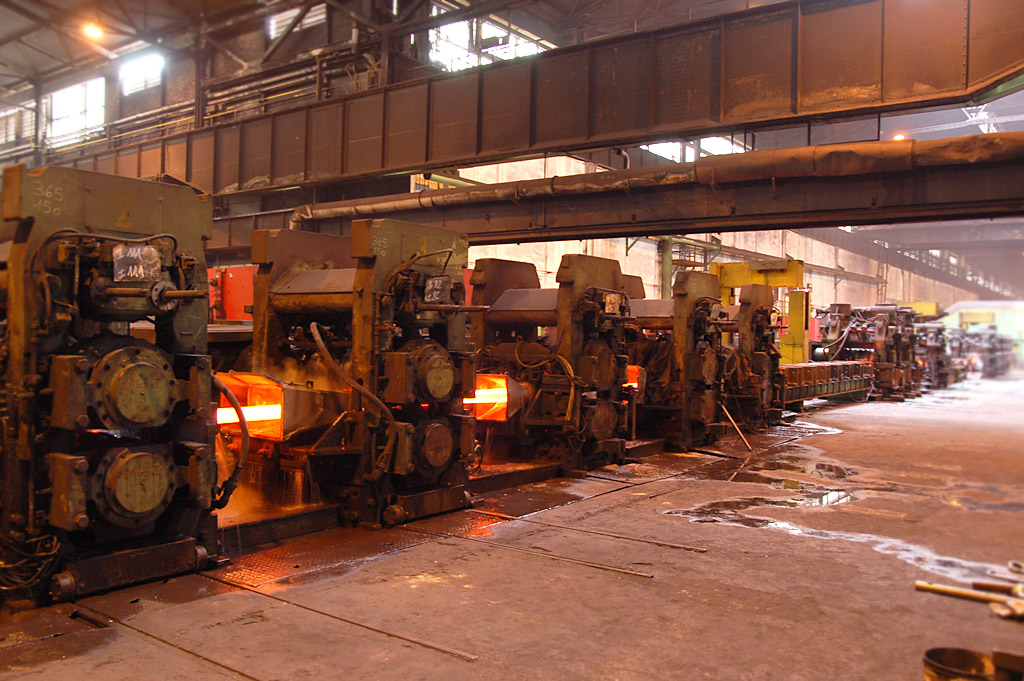
\includegraphics[height=2.5cm]{png/laminoirs}
\textit{Train de laminoirs}
\end{center}
\end{minipage} \hfill
\begin{minipage}[c]{.2\linewidth}
\begin{center}
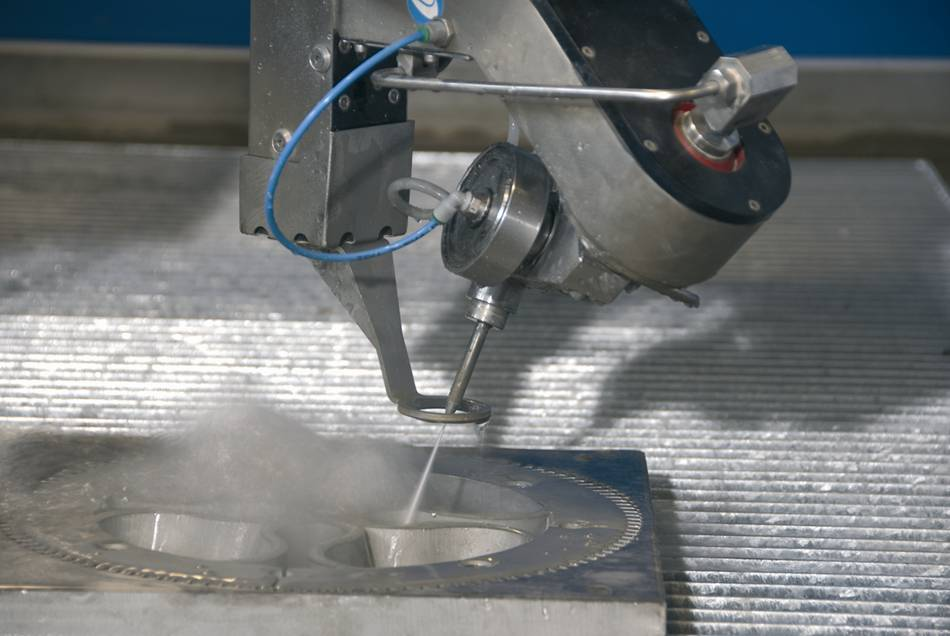
\includegraphics[height=2.5cm]{png/jetdeau}

\textit{Découpe au jet d'eau}
\end{center}
\end{minipage} \hfill
\begin{minipage}[c]{.2\linewidth}
\begin{center}
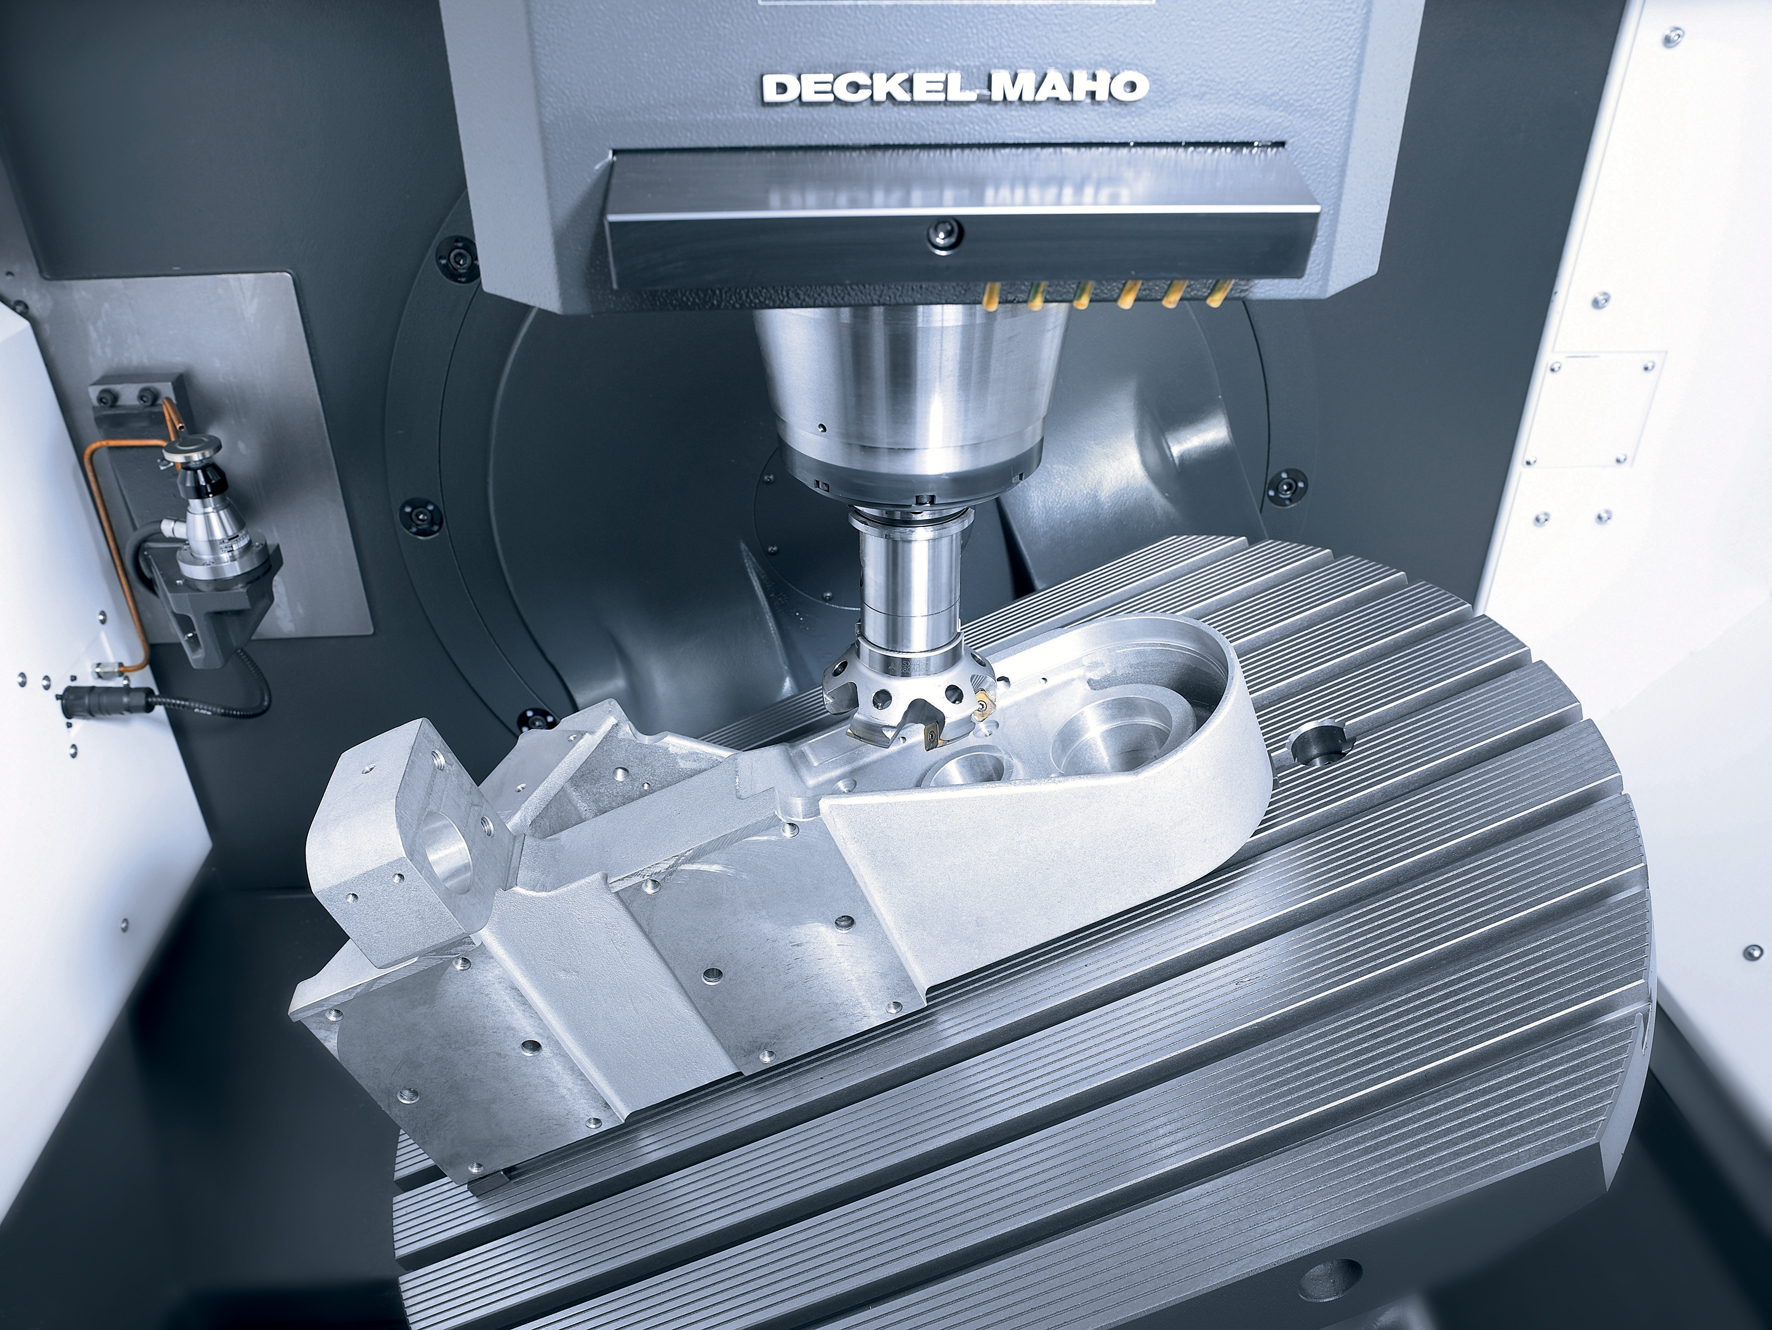
\includegraphics[height=2.5cm]{png/5axes}

\textit{Usinage sur centre UGV 5 axes}
\end{center}
\end{minipage} \hfill
\begin{minipage}[c]{.2\linewidth}
\begin{center}
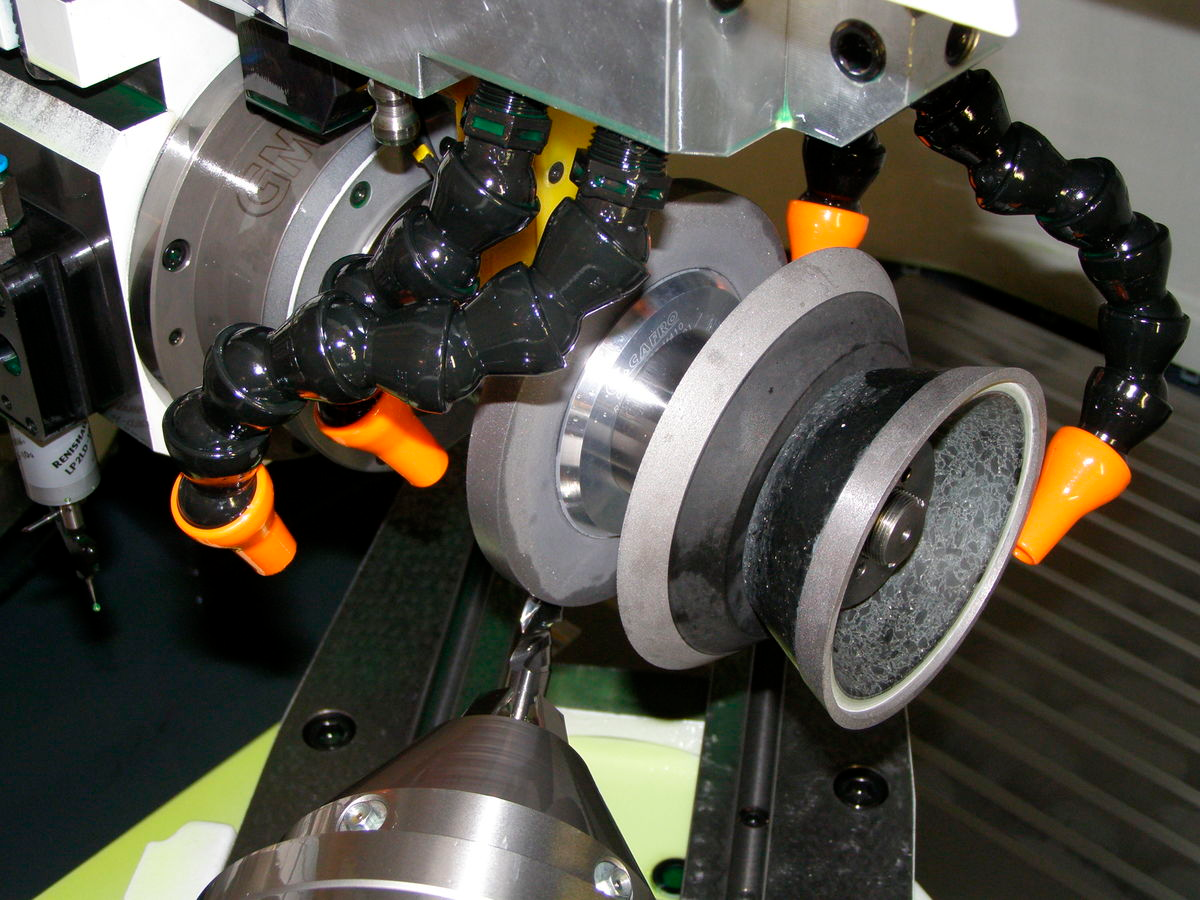
\includegraphics[width=.9\textwidth]{png/rectif.png}

\textit{Rectification d'une fraise avec meule diamantée}
\end{center}
\end{minipage}

\vspace{.5cm}



Les pièces que nous sommes amenés à concevoir sont destinées, tôt ou tard, à être fabriquées. Le but de ce cours est d'aborder, de manière générale un certain nombre de procédés qui permettent de fabriquer une pièce. De manière générale, plusieurs procédés différents interviennent dans la réalisation d'une pièce. Vous devrez alors être capables de citer l'ensemble de ces procédés.


%\begin{center}
%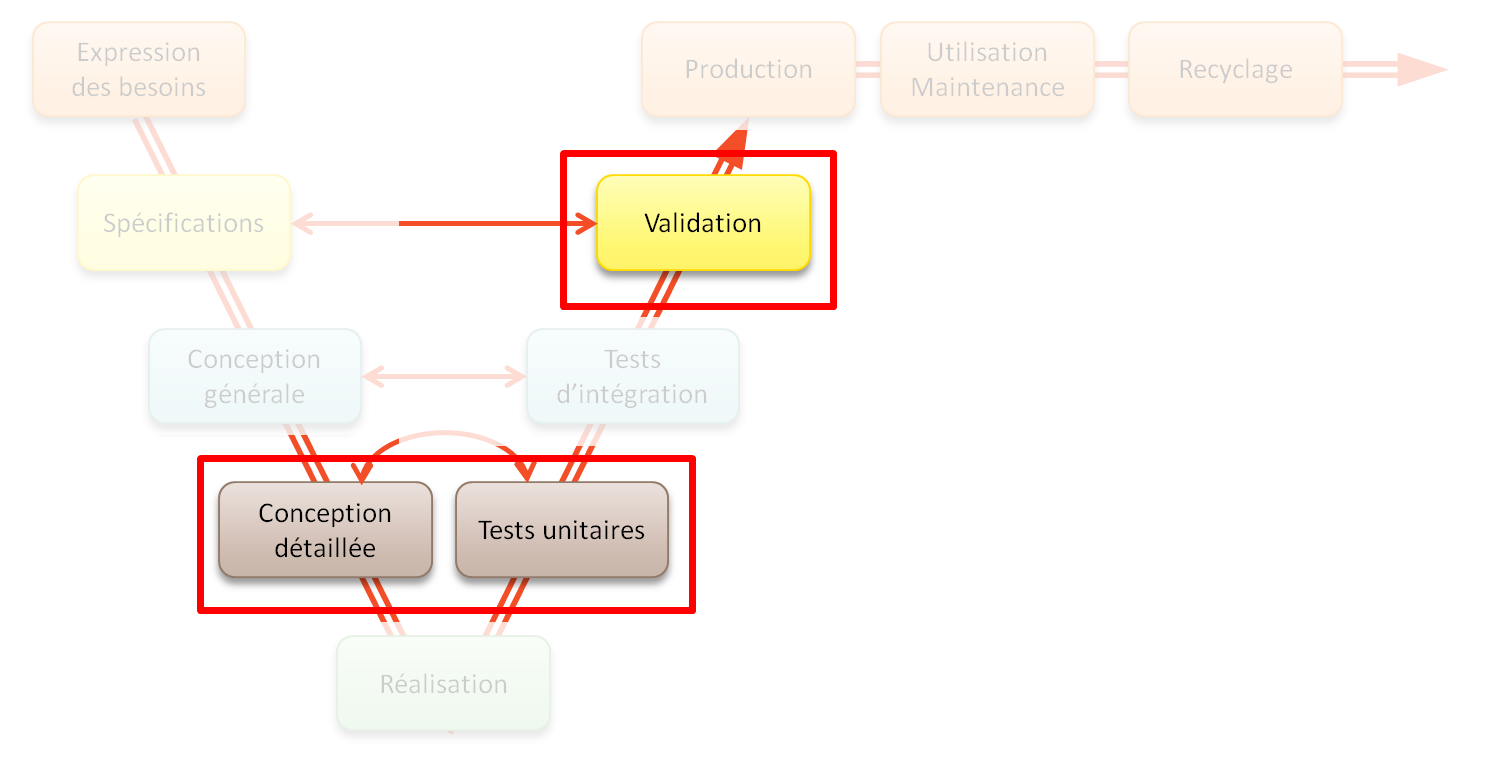
\includegraphics[width=.9\textwidth]{png/cyclev.png}

%\textit{Cycle de conception d'un produit}
%\end{center}

%\begin{prob}
%\textsc{Problématique :}

%En phase d'avant conception d'un produit, quels sont les critères qui vont permettre de choisir les matériaux à utiliser ?
%\end{prob}

\begin{savoir}
\textsc{Savoirs :}
\begin{itemize}
\item Connaître des modes d'obtention des pièces.
\end{itemize}
\end{savoir}

%\newpage 

\setlength{\parskip}{0ex plus 0.2ex minus 0ex}
 \renewcommand{\contentsname}{}
 \renewcommand{\baselinestretch}{1}

\tableofcontents

 \renewcommand{\baselinestretch}{1.2}
\setlength{\parskip}{2ex plus 0.5ex minus 0.2ex}

% \vspace{1cm}
\textit{Ce document évolue. Merci de signaler toutes erreurs ou coquilles.}

%\newpage

\section{Procédés d'élaboration des pièces brutes}
\subsection{Obtention des bruts par déformation plastique}
\subsubsection{Le laminage}
\begin{minipage}[c]{.55\linewidth}
Le laminage est un procédé qui permet d'obtenir des feuilles ou des profilés de géométrie variée, mais de section pleine. 

En général, le laminage est réalisé à partir de lingots provenant des hauts fourneaux qui ont été préalablement chauffés. On parle alors de laminage à chaud. Ces lingots passent alors entre des cylindres afin d'obtenir la pièce souhaitée. 
\end{minipage} \hfill
\begin{minipage}[c]{.4\linewidth}
\begin{center}
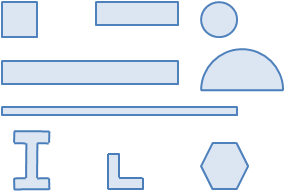
\includegraphics[width=0.9\textwidth]{png/profiles}
\end{center}
\end{minipage}
\begin{center}
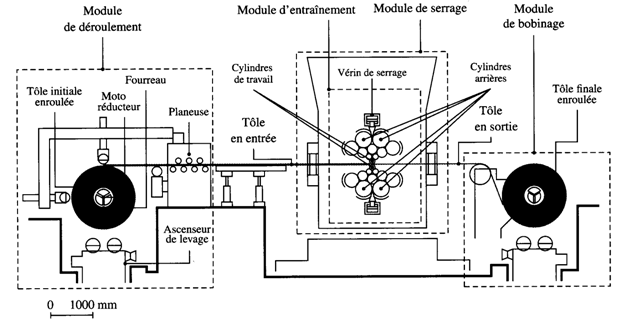
\includegraphics[width=0.9\textwidth]{png/laminoir}
\end{center}

\subsubsection{Le forgeage}
\begin{minipage}[c]{.3\linewidth}
\begin{center}
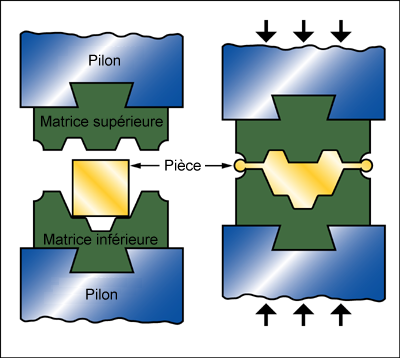
\includegraphics[width=0.9\textwidth]{png/forge_schema}
\end{center}
\end{minipage}\hfill
\begin{minipage}[c]{.65\linewidth}
Le forgeage consiste en déformer un lopin par chocs successifs grâce à un marteau pilon. Parmi les procédés de forge existants, on peut distinguer : 
\begin{itemize}
\item la forge libre;
\item la forge par estampage (forgeage de métaux ferreux);
\item la forge par matriçage (forgeage de métaux non ferreux).
\end{itemize}

La déformation du lopin peut se faire à chaud ou à froid. En forge par estampage, il est nécessaire de concevoir une série de matrices qui vont permettre de réaliser le brut désiré. 
\end{minipage}

\begin{minipage}[c]{.3\linewidth}
\begin{center}
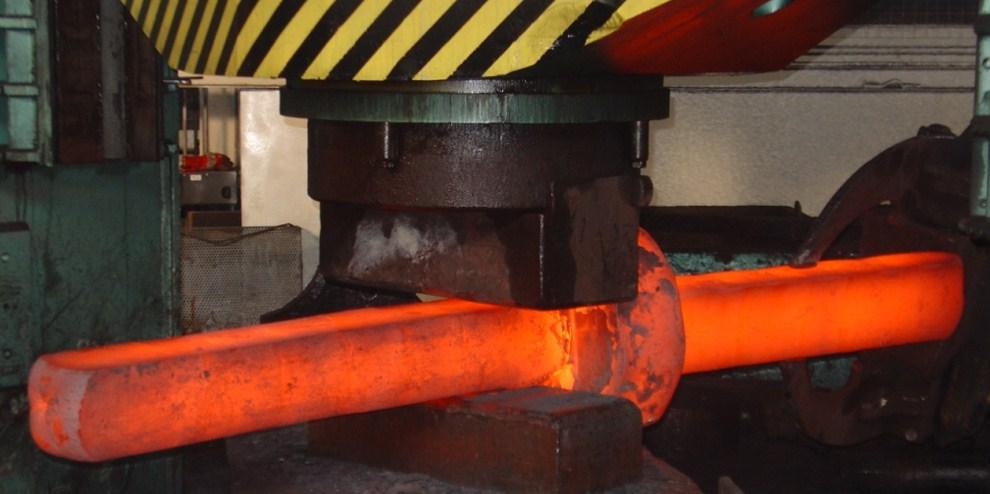
\includegraphics[height=3cm]{png/forge_libre}

\textit{Forge libre d'un arbre à section carrée \cite{forgelibre}}
\end{center}
\end{minipage}\hfill
\begin{minipage}[c]{.3\linewidth}
\begin{center}
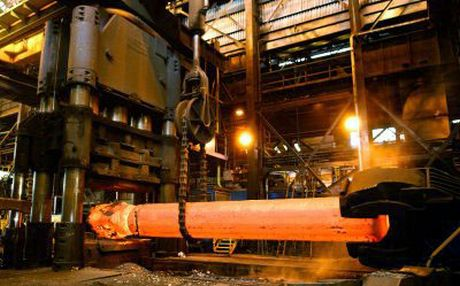
\includegraphics[height=3cm]{png/forge}

\textit{Forge}
\end{center}
\end{minipage}\hfill
\begin{minipage}[c]{.3\linewidth}
\begin{center}
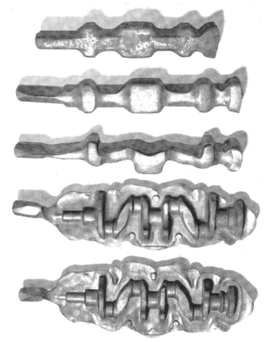
\includegraphics[width=0.7\textwidth]{png/estampage}

\textit{Étapes de forgeages menant à la fabrication d'un vilebrequin}
\end{center}
\end{minipage}

\subsubsection{L'extrustion}

L'extrusion est un procédé au cours duquel on oblige la matière à passer dans  un orifice de section déterminée. 


\begin{minipage}[c]{.3\linewidth}
\begin{center}
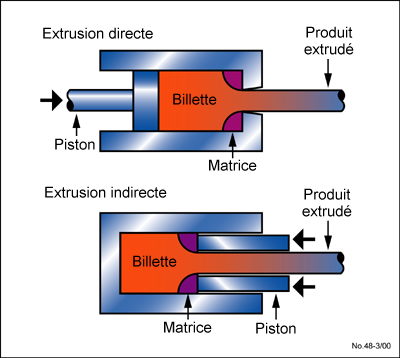
\includegraphics[height=4cm]{png/extrusion_schema}
\end{center}
\end{minipage}\hfill
\begin{minipage}[c]{.3\linewidth}
\begin{center}
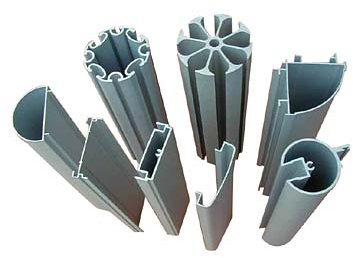
\includegraphics[height=4cm]{png/profils_extrudes}

\textit{Profils en aluminium extrudés \cite{extrusion}}
\end{center}
\end{minipage}\hfill
\begin{minipage}[c]{.3\linewidth}
\begin{center}
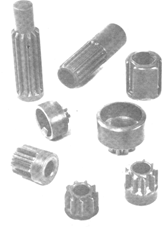
\includegraphics[height=4cm]{png/profils_extrudes2}
\end{center}
\end{minipage}



%\subsubsection{Mise en forme des métaux en feuille}
%\subsubsection{Le cisaillage}
\subsubsection{Le découpage}
Découper des matériaux en feuille, d'épaisseur plus ou moins importante est souvent le préalable à la réalisation d'une pièce. Plusieurs techniques se font concurrence.

\paragraph*{Découpe par jet d'eau}

\begin{minipage}[c]{.25\linewidth}
\begin{center}
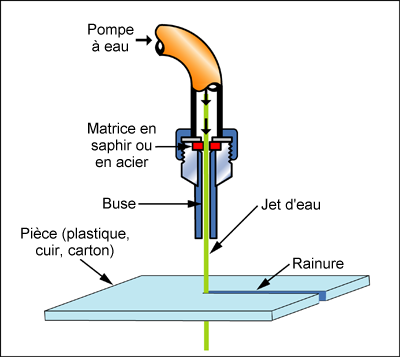
\includegraphics[width=.9\textwidth]{png/jeteau}
\end{center}
\end{minipage} \hfill
\begin{minipage}[c]{.6\linewidth}
A l'aide d'une buse on projette un fin jet d'eau à très haute pression. La sortie de la buse se fait alors autour de la vitesse de 900m/s. L'eau peut être chargée avec des abrasifs.

Ce procédé permet la découpe de matériaux épais (>100 mm) et de composites. Il n'y a pas de chaleur et d'échauffement, pas de gaz et de vapeurs toxiques, pas ou peu de déformations et pas de limites dans la forme des découpes. 
	
Par contre on ne peut découper des corps creux dans de bonnes conditions, la précision est moyenne, délaminage possible, humidité ambiante, usure des buses.

Le pilotage de la buse peut être manuel ou à commande numérique.
\end{minipage}

\paragraph*{Découpe au laser}
\begin{minipage}[c]{.25\linewidth}
\begin{center}
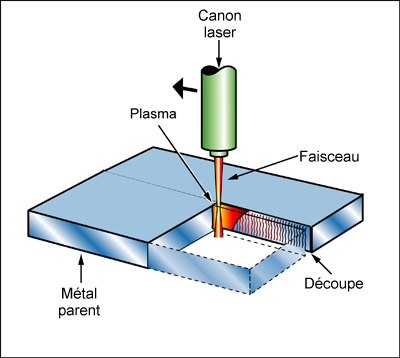
\includegraphics[width=.9\textwidth]{png/laser}
\end{center}
\end{minipage} \hfill
\begin{minipage}[c]{.6\linewidth}
On utilise dans ce cas l'énergie thermique d'un faisceau laser.

Ce procédé permet une grande vitesse d'avance et un travail précis, la largeur de saignée est réduite, il n'y a pas d'usure et peu de limites dans les formes découpées, il y a peu de déformations.

Certains métaux réfléchissants ne peuvent être découpés (Cu, Au, ...). On ne peut couper les corps creux et multicouches. Il y a émission de gaz toxiques et la matière peut être thermiquement affectée. 

Le procédé reste cher par son installation. Le pilotage peut être manuel ou à commande numérique.
\end{minipage} 

\paragraph*{Electroérosion par fil}
\begin{minipage}[c]{.25\linewidth}
\begin{center}
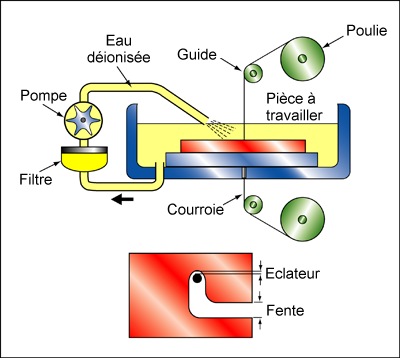
\includegraphics[width=.9\textwidth]{png/fil}
\end{center}
\end{minipage} \hfill
\begin{minipage}[c]{.6\linewidth}
On utilise la microfusion de la matière due à l'arc électrique se produisant entre le fil et la matière.

On peut réaliser des découpes très épaisses (>400 mm), avec des dépouilles ($30^{\text{o}}$), avec une grande précision ($5\; \mu m$). La découpe de nids d'abeille est possible.

Par contre le procédé est lent, les courses limitées et le matériau doit être conducteur.
\end{minipage}

\paragraph*{Oxycoupage}
\begin{minipage}[c]{.25\linewidth}
\begin{center}
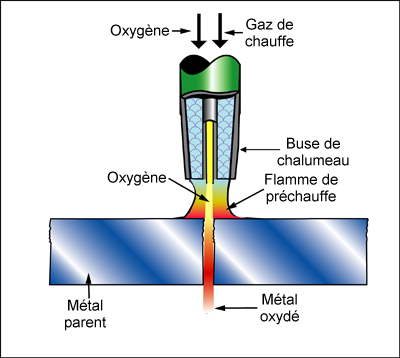
\includegraphics[width=.9\textwidth]{png/oxycoupage}
\end{center}
\end{minipage} \hfill
\begin{minipage}[c]{.6\linewidth}
Utilisation de l'action d'un jet d'oxygène sur de l'acier chauffé. Permet des découpes simples sur des tôles en acier pouvant aller jusqu'à 6 m d'épaisseur.
\end{minipage} 

\subsubsection{Le pliage}
Sur une portion de tôle appelée flan on exerce à l'aide d'un outil de forme variée un effort sur une pièce reposant sur quelques appuis. Cet effort déforme le flan dans le domaine plastique. Ci dessous sont données quelques configurations de pliage. Le domaine d'application est vaste et trouve toute son application dans des secteurs comme l'électroménager.

\begin{center}
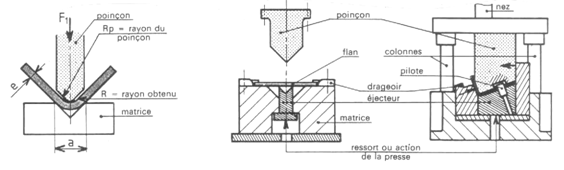
\includegraphics[width=0.7\textwidth]{png/pliage}
\end{center}

\subsubsection{L'emboutissage}

\begin{minipage}[c]{.65\linewidth}
En emboutissage la déformation peut être qualifiée de tridimensionnelle. Les formes obtenues sont rarement développables. L'application type est la réalisation des pièces de carrosserie automobile.

\end{minipage}\hfill
\begin{minipage}[c]{.3\linewidth}
\begin{center}
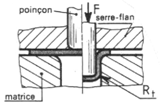
\includegraphics[width=0.9\textwidth]{png/emboutissage1}
\end{center}
\end{minipage}

\begin{center}
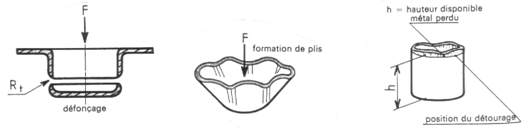
\includegraphics[width=0.7\textwidth]{png/emboutissage2}
\end{center}

\subsubsection{Le poinçonnage}
\begin{minipage}[c]{.65\linewidth}
L'image la plus simple est donnée par la perforatrice des écoliers. La forme du poinçon définit la forme des pièces que l'on peut obtenir et il n'y a guère de limite à sa forme.

\end{minipage}\hfill
\begin{minipage}[c]{.3\linewidth}
\begin{center}
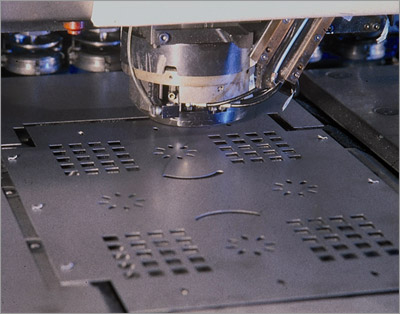
\includegraphics[width=0.9\textwidth]{png/poinconnage}
\end{center}
\end{minipage}



\subsection{Obtention des bruts à partir de métaux liquides}
L'ensemble des procédés de moulage impose une contrainte de matériau et une contrainte de moule. Le matériau liquide doit pouvoir remplir intégralement le moule et doit pouvoir se refroidir de façon homogène pour éviter des défauts. Le moule doit permettre le démoulage, soit par sa destruction (il faut alors pouvoir en refaire un autre facilement), soit par sa conception (angles de dépouille, arrondis, plan de joint). Il est donc nécessaire de parler :
\begin{itemize}
\item du moulage au sable avec moule non permanent;
\item du moulage en coquille métallique;
\item du moulage à cire perdue.
\end{itemize}

\subsubsection{Moule destructible, modèle non destructible -- Fonderie au sable}
\begin{rem}
Dans ce procédé on détruit le moule donc aucun problème pour récupérer la pièce MAIS il faut sortir le modèle de l'empreinte en sable : il y a donc un problème de démoulage.
\end{rem}


\begin{minipage}[c]{.3\linewidth}
\begin{center}
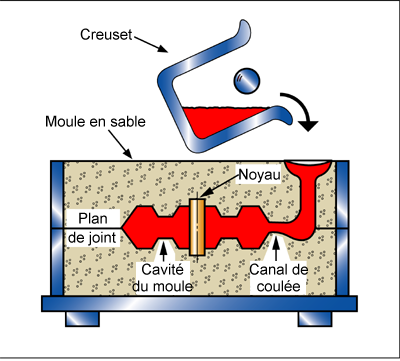
\includegraphics[width=0.9\textwidth]{png/moulage}
\end{center}
\end{minipage}\hfill
\begin{minipage}[c]{.65\linewidth}

Le moulage à modèle pemanent et moule non permanent est très répandu dans l'industrie. Il permet par exemple d'obtenir les blocs moteurs de voiture, les disques de freins \textit{etc}.

Le moule est réalisé en sable. La haute température de fusion du sable permet de mouler des pièces en fonte ou en acier. 
\begin{rem}
De manière générale on évitera de mouler des pièces en acier. Le moulage sera davantage utilisé pour les pièces en fonte ou en alliage d'aluminium.
\end{rem}

\end{minipage}

Les procédés de moulage feront l'objet d'un cours supplémentaire. Voici un résumé des étapes permettant d'arriver à la fabrication d'un produit : 
\begin{enumerate}
\item Les formes extérieures de la pièces sont réalisées sur une pièce appelée modèle (par exemple en bois). Il est composé d'au moins 2 demi modèles.
\item Les formes intérieures de la pièces sont réalisées sur une pièce appelée noyau (en sable).
\item Le demi modèle est positionné dans un demi-châssis, face contre table. On va alors tasser du sable autour du modèle.
\item La plaque est retournée. On y adjoint le second modèle et le second châssis ainsi que les organes de coulée. On tasse du sable autour du second demi modèle.
\item On ouvre les châssis pour retirer le modèle. 
\item On positionne le noyau. 
\item On referme le moule. 
\item On peut alors couler la pièce.
\item Une fois le métal refroidi, on casse le moule en sable ainsi que le noyau pour récupérer la pièce.
\end{enumerate}




\subsubsection{Moule non destructible}

\begin{minipage}[c]{.3\linewidth}
\begin{center}
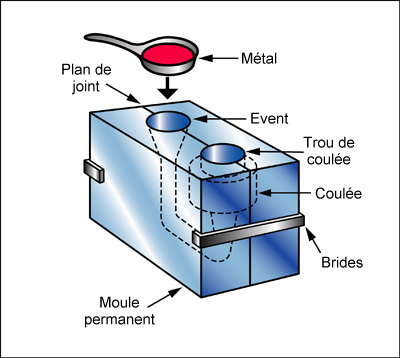
\includegraphics[width=0.9\textwidth]{png/moulage2}
\end{center}
\end{minipage}\hfill
\begin{minipage}[c]{.65\linewidth}
Le procédé de moulage en coquille consiste en réaliser un moule, généralement an acier. Un métal est coulé dans le moule. Une fois le métal refroidi, on ouvre le moule pour récupérer la pièce. Dans ce type de moulage, il est nécessaire que la température de fusion de la pièce soit inférieur à la température de fusion du moule. 
\end{minipage}

\subsubsection{Moule destructible, modèle destructible -- Moulage à la cire perdue}

Le moulage à la cire perdue est souvent utilisé pour des séries importantes de petites pièces.
Un modèle en cire est généralement obtenu en grappe, par moulage. La grappe de modèle est ensuite recouverte de sable, ou de platre. Lors du coulage du métal dans le moule, la cire fond et laisse place au métal. On récupère ensuite les pièces par destruction du moule.

\begin{minipage}[c]{.45\linewidth}
\begin{center}
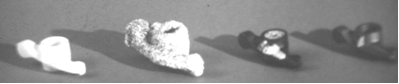
\includegraphics[width=0.95\textwidth]{png/cire1}
\end{center}
\end{minipage} \hfill
\begin{minipage}[c]{.45\linewidth}
\begin{center}
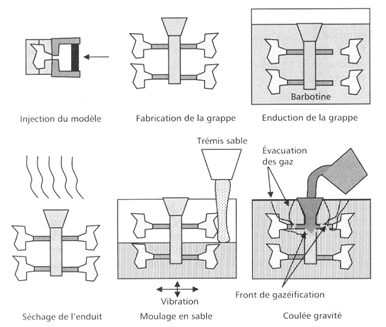
\includegraphics[width=0.95\textwidth]{png/cire2}
\end{center}
\end{minipage}

\subsection{Obtention des bruts à partir de métaux en poudre}
\begin{minipage}[c]{.35\linewidth}
\begin{center}
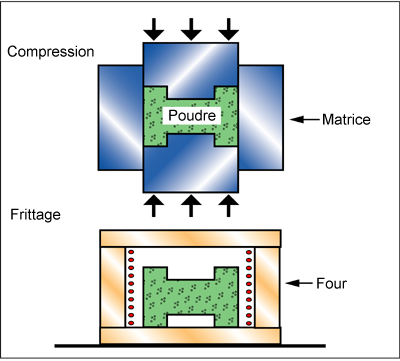
\includegraphics[width=0.95\textwidth]{png/frittage}
\end{center}
\end{minipage} \hfill
\begin{minipage}[c]{.55\linewidth}
Le frittage est utilisé pour mettre en forme des poudres (par exemple des céramiques). La poudre est mise dans un moule puis chauffée à une température inférieure à la température de fusion. Sous l'effet de la chaleur et grâce au phénomène de diffusion, la poudre va s'agglomérer pour former une pièce.

\begin{exemple}
Les coussinets en bronze sont obtenus par frittage. La pièce obtenue possède des porosités qui vont être comblées par de l'huile. Lors du fonctionnement l'huile est restituée assurant ainsi la lubrification du coussinet.
\end{exemple}
\end{minipage}

\subsection{Assemblage par soudage}

Souder c'est assembler de façon définitive une ou plusieurs pièces en assurant entre elles la continuité de la matière. 

Le soudo-brasage et le brasage : l'assemblage est hétérogène, la formation du joint ou cordon est assurée par la seule intervention du métal d'apport qui agit comme une colle. La température de fusion du métal d'apport est inférieure à celle des matériaux à souder qui peuvent être de natures différentes.
	
Le soudage autogène : les pièces à assembler, de même nature ou de composition voisine, participent à la constitution du joint ou du cordon de soudure. L'assemblage est dit homogène.


\begin{minipage}[c]{.45\linewidth}
\begin{center}
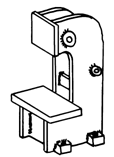
\includegraphics[width=0.3\textwidth]{png/soudage1}

\textit{Réalisation d'un bâti à partir de tôles plates} 
\end{center}
\end{minipage}\hfill
\begin{minipage}[c]{.45\linewidth}
\begin{center}
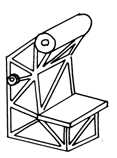
\includegraphics[width=0.3\textwidth]{png/soudage2}

\textit{Réalisation d'un bâti à partir de profilés} 
\end{center}
\end{minipage}


\subsubsection{Le soudage à l'arc}
\begin{minipage}[c]{.3\linewidth}
\begin{center}
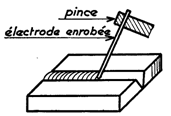
\includegraphics[width=0.9\textwidth]{png/arc}
\end{center}
\end{minipage}\hfill
\begin{minipage}[c]{.65\linewidth}

L'électrode ne touche pas la pièce. Un arc électrique se crée.

La baguette fond ainsi que les pièces à assembler.

L'enrobage de la baguette constitue le laitier qui permet de protéger la soudure avant son refroidissement 

\end{minipage}


\subsubsection{Le soudage par point}

\begin{minipage}[c]{.3\linewidth}
\begin{center}
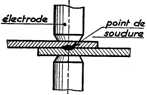
\includegraphics[width=0.9\textwidth]{png/points}
\end{center}
\end{minipage}\hfill
\begin{minipage}[c]{.65\linewidth}

Assemblage de tôles : le passage du courant entraîne un point de fusion puis effort de serrage pour assurer l'interpénétration.

\end{minipage}

\subsubsection{Le soudage au chalumeau}

\begin{minipage}[c]{.3\linewidth}
\begin{center}
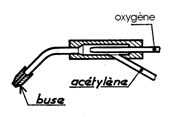
\includegraphics[width=0.9\textwidth]{png/chalumeau}
\end{center}
\end{minipage}\hfill
\begin{minipage}[c]{.65\linewidth}

Chaleur obtenue par combustion d'oxygène et d'acétylène ($>\; 1\,800^{\text{o}}$)

\end{minipage}

\section{Procédés de finition des pièces}
Dans ces procédés il y a toujours combinaison de deux mouvements. L'un de puissance importante destiné à enlever la matière, appelé mouvement de coupe l'autre, de puissance moindre destiné à déplacer la pièce pour l'obtention des divers profils usinés, le mouvement d'avance.
	
D'autre part si l'outil laisse l'image de sa forme sur la pièce on parle d'un travail de forme, si la forme créée est la résultante de la trajectoire d'un point particulier de l'outil on parle de travail d'enveloppe ou de travail par génération. 

Avec l'usinage par enlèvement de métal on peut obtenir sans difficulté des travaux en série de qualité 8. Les travaux de qualité 7 demanderont des précautions particulières.

\begin{center}
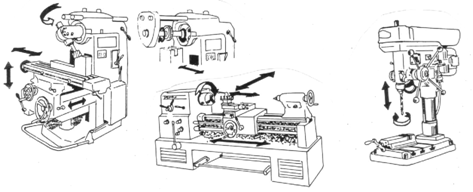
\includegraphics[width=0.7\textwidth]{png/usinage}

\textit{Principaux mouvements des machines usuelles}
\end{center}

\subsection{Le tournage}

L'usinage est une combinaison d'un mouvement de coupe et un mouvement d'avance. Dans le cas du tournage, la pièce est entraînée en rotation, générant ainisi le mouvement de coupe. L'outil est lui animé de mouvements de translation. Le tournage (2 axes) permet d'obtenir des pièces de révolution. 


\begin{center}
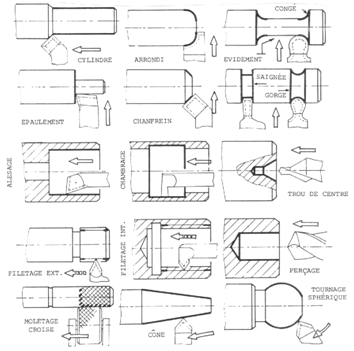
\includegraphics[width=0.5\textwidth]{png/tournage}
\end{center}

\subsection{Le fraisage}

Dans le cas du fraisage, l'outil (fraise) est animé d'un mouvement de rotation. Le déplacement de la fraise permet de réaliser tout type de pièces. 
\begin{center}
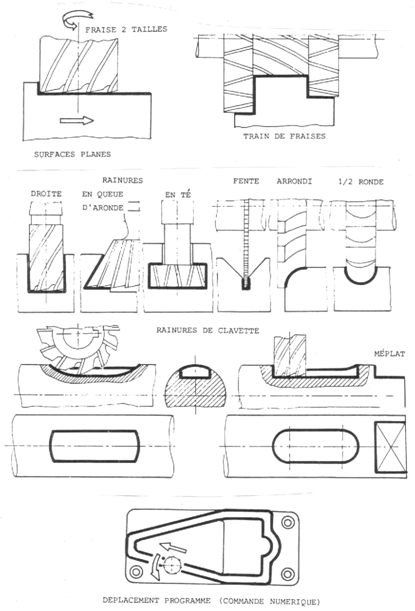
\includegraphics[width=0.5\textwidth]{png/fraisage}
\end{center}

\subsection{Le perçage -- alésage}

\begin{center}
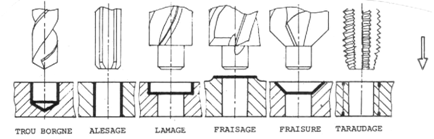
\includegraphics[width=0.6\textwidth]{png/percage}
\end{center}


\subsection{Le brochage}
\begin{minipage}[c]{.45\linewidth}
\begin{center}
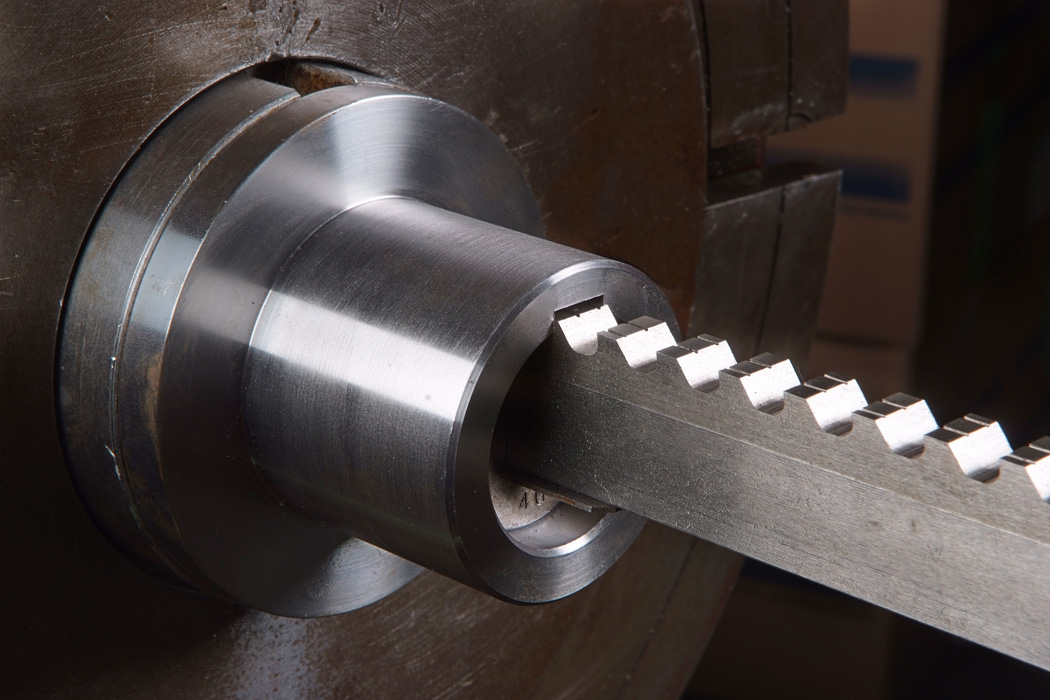
\includegraphics[width=.5\textwidth]{png/brochage1}
\end{center}
\end{minipage} \hfill
\begin{minipage}[c]{.45\linewidth}
\begin{center}
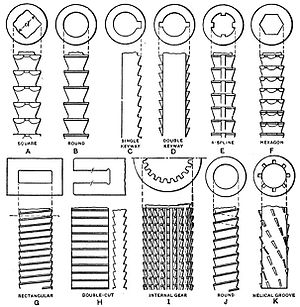
\includegraphics[width=.5\textwidth]{png/brochage2}
\end{center}
\end{minipage} 
\subsection{Les procédés de finition}
\subsubsection{La rectification}
L'usinage se fait ici par abrasion.

La meule est constituée d'une multitude de grains d'abrasif (oxyde d'alumine) réunis par un agglomérant. Ces grains se comportent comme autant de micro-outils.

Quand ils sont usés, les forces s'exerçant sur ces grains sont suffisantes pour en permettre l'extraction. Des grains neufs entrent alors en action. 

Une meule qui usine s'use et doit être régénérée par un diamantage.


\begin{center}
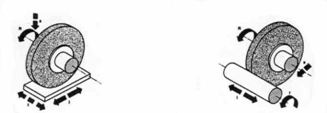
\includegraphics[width=0.5\textwidth]{png/rectif1}

\textit{Rectification plane et cylindrique}
\end{center}

\begin{minipage}[c]{.45\linewidth}
La rectification permet en série d'obtenir la qualité 7 voire la qualité 6. 

Il est évident qu'elle nécessite une ébauche usinée préalable pour avoir peu de matière à enlever et surtout faire travailler les meules sur une surface homogène.

Le tableau ci-contre donne quelques configurations de rectification.


\end{minipage}\hfill
\begin{minipage}[c]{.5\linewidth}
\begin{center}
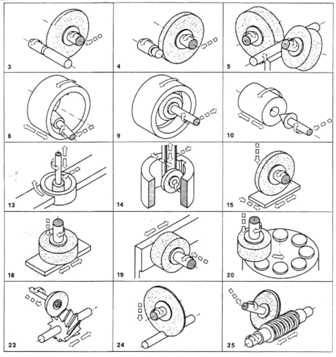
\includegraphics[width=0.9\textwidth]{png/rectif2}
\end{center}
\end{minipage}


%\subsubsection{Le polissage}




\begin{thebibliography}{2}
%\bibitem{zwick}{\url{http://www.zwick.fr/fr.html}}

%\bibitem{acier}{\url{http://www.lefigaro.fr/medias/2008/12/18/47e0e366-cd2c-11dd-882f-4b99bc2f9b71.jpg}}
%\bibitem{composite}{\url{http://fr.gurit.com/benefits-of-composite-materials.aspx}}
%\bibitem{verre}{\url{http://www.vezenobres.info/partenaires.htm}}
%\bibitem{ldr}{LDR Médical \url{http://fr.ldrmedical.com/Produits/Thoraco-lombaire/MobidiscProthèsededisquelombaire}}
%\bibitem{dent}{Protilab \url{http://www.protilab.com/fr/prothese/7/Couronne+sur+implant}}
%\bibitem{wafer}{\url{http://www.efficacite-electrique.fr/2012/03/usa-semi-conducteurs-plus-compacts-meilleure-efficacite-electrique/}}
%\bibitem{carter}{\url{http://www.directindustry.fr/prod/sermes/moto-reducteurs-electriques-a-vis-sans-fin-a-carter-en-fonte-7542-424078.html}}
%\bibitem{fer}{\url{http://www.zpag.net/Tecnologies_Indistrielles/Metaux_Ferreux.htm}}
%\bibitem{a350}{© Airbus S.A.S.}

\bibitem{forgelibre}{Forge libre -- \url{http://www.union-des-forgerons.fr/fr/activite/forge}}
\bibitem{extrusion}{Extrusion de profils d'aluminium -- \url{http://lakealjin.en.supplierlist.com/product_view/lakealjin/189472/101212/aluminum_extrusion_profile.htm}}
%\bibitem{rb}{Supports de cours de Renan Bonnard,PTSI, Lycée Newton, Clichy la Garenne}
%\bibitem{jb}{Supports de cours de Joël Boiron, PTSI, Lycée Gustave Eiffel, Bordeaux}}
%\bibitem{mc}{Supports de cours de Maryline Carrez, Lycée Jules Haag, Besançon}
%\bibitem{pf}{Supports de cours de Philippe Fichou, Lycée Vauban, Brest \url{http://philippe.fichou.pagesperso-orange.fr/documents/liaisoncomplete2003.pdf}}
\bibitem{jpp}{Supports de cours de Jean-Pierre Pupier, Lycée Rouvière, Toulon}


\end{thebibliography}

\end{document}